%\usepackage{flafter}  % Don't place floats before their definition


\chapter{\label{chap:localExpansion}Local Expansion of Nonlocal Interactions}


I investigate the validity of expanding a nonlocal scalar potential $V(\vecrp,\vec{r})$ around a small nonlocality, i.e. when the potential is nearly diagonal in $|\vec{r}-\vecrp|$. 


\begin{section}{Expanding the nonlocal potential}
A two-body nonlocal potential takes the form $V(\vecrp,\vec{r})$ and the coordinate dependent part may be evaluated as
\begin{equation}\label{eqn:nonlocaldef}
\braket{n' l' m'| V | n l m}=\int d^3r\:d^3r'\:R^*_{n',l'}(r') Y^*_{l',m'}(\hat{r}') V(\vecrp,\vec{r}) R_{n,l}(r) Y_{l,m}(\hat{r}).
\end{equation}
Throughout, we will assume that the potential is a scalar operator. Because nonlocal potentials require greater computational resources, it would be desirable to find a suitable local approximation. Intuitively, we can imagine that the potential $V(r,r')$ is nearly local. We take this to mean that it the contribution to the matrix element is small when $\vec{r}-\vecrp$ is large. We thus make a coordinate change with unit Jacobian to \eqref{eqn:nonlocaldef}. A suitable choice of coordinates is the linear combination
\begin{equation}\label{eqn:coords}
\vec{r}_1=\frac{\vec{r}+\vecrp}{2},\vec{r}_2=\vec{r}-\vecrp
\end{equation}
for which our nonlocality condition reduces to the requirement that the potential falls off rapidly in $r_2$. In the interest of generating clear, compact expressions we will also use the convenient definitions
\begin{align}
F(\vecrp)&=R^*_{n',l'}(r') Y^*_{l',m'}(\hatrp)\\
G(\vec{r})&=R_{n,l}(r) Y_{l,m}(\hat{r})
\end{align}
In these coordinates, the matrix elements become 
\begin{equation}
\bra{n' l' m'} V \ket{ n l m}= \int d^3r_1\:d^3r_2\:F\left( \vec{r}_1-\frac{\vec{r}_2}{2} \right) V\left(\vec{r}_1-\frac{\vec{r}_2}{2},\vec{r}_1+\frac{\vec{r}_2}{2}\right) 
G\left( \vec{r}_1+\frac{\vec{r}_2}{2}\right).
\end{equation}
We then make a Taylor expansion of the wave functions $F$ and $G$ in the coordinate $\vec{r}_2$ (not the potential itself). The three dimensional Taylor expansion can be written in Cartesian form as
\begin{align}\label{eq:TaylorExpansion}
F\left(\vec{r}_1-\frac{\vec{r}_2}{2}\right)&=F(\vec{r}_1)-\frac{1}{2}\vec{r}_2\cdot\vec{\nabla}_1 F(\vec{r}_1)+\frac{1}{2}\left(\frac{1}{2}\vec{r}_2\cdot\vec{\nabla}_1\right)\left(\frac{1}{2}\vec{r}_2\cdot\vec{\nabla}_1\right)F(\vec{r}_1)+\dots 
\\
G\left(\vec{r}_1+\frac{\vec{r}_2}{2}\right)&=G(\vec{r}_1)+\frac{1}{2}\vec{r}_2\cdot\vec{\nabla}_1 G(\vec{r}_1)+\frac{1}{2}\left(\frac{1}{2}\vec{r}_2\cdot\vec{\nabla}_1\right)\left(\frac{1}{2}\vec{r}_2\cdot\vec{\nabla}_1\right)G(\vec{r}_1)+\dots
\end{align}
Note that the asymmetric choice of coordinates made in \eqref{eqn:coords} has the desirable effect of allowing one to expand the wave functions around $\vec{r}_1$ without any additional constants. Compare this expansion also with that of \cite{0954-3899-26-3-310}, where only the function $G(\vec{r})$ is expanded around $\vec{r}=\vecrp$. Plugging this expansion in up to second order 
\begin{equation}\label{eqn:expansionCartesian}
\begin{split}
\braket{n' l' m'| V | n l m} &= \int d^3r_1\: F(\vec{r}_1)\left[\int d^3r_2\:\left\{V\left(\vec{r}_1-\frac{\vec{r}_2}{2},\vec{r}_1+\frac{\vec{r}_2}{2}\right) \right.\right. \\
&-\frac{1}{2} \left(\lvec{\nabla}_1\cdot\vec{r}_2\: V\left(\vec{r}_1-\frac{\vec{r}_2}{2},\vec{r}_1+\frac{\vec{r}_2}{2}\right) -
V\left(\vec{r}_1-\frac{\vec{r}_2}{2},\vec{r}_1+\frac{\vec{r}_2}{2}\right) \vec{r}_2\cdot\vec{\nabla}_1
\right)\\
&-\frac{1}{4}\lvec{\nabla}_1\cdot\vec{r}_2\: V\left(\vec{r}_1-\frac{\vec{r}_2}{2},\vec{r}_1+\frac{\vec{r}_2}{2}\right) \vec{r}_2\cdot\vec{\nabla}_1\\
&+\frac{1}{8}\left(\lvec{\nabla}_{1}\cdot\vec{r}_2\right)^2 V\left(\vec{r}_1-\frac{\vec{r}_2}{2},\vec{r}_1+\frac{\vec{r}_2}{2}\right) 
\left.\left.+\frac{1}{8} V\left(\vec{r}_1-\frac{\vec{r}_2}{2},\vec{r}_1+\frac{\vec{r}_2}{2}\right) \left(\vec{r}_2\cdot\vec{\nabla}_{1}\right)^2+\dots \right\}\right]G(\vec{r}_1)
\end{split}
\end{equation}

Alternately, we can also express the expansion \eqref{eq:TaylorExpansion} in terms of spherical tensor operators,
\begin{align}
\begin{split}
F\left(\vec{r}_1-\frac{\vec{r}_2}{2}\right)=
F(\vec{r}_1)&-\frac{1}{2}\sqrt{\frac{4\pi}{3}}\sum_{m}(-1)^m r_2 Y_{1,m}(\hat{r}_2) \vec{\nabla}_{1,-m} F(\vec{r}_1) \\
&\hspace{.5cm}+\frac{1}{8}\frac{4\pi}{3}\sum_{m,m'}(-1)^{m+m'}r_2^2 Y_{1,m}(\hat{r}_2)Y_{1,m'}(\hat{r}_2)\vec{\nabla}_{1,-m}\vec{\nabla}_{1,-m'}F(\vec{r}_1)
+\dots 
\end{split}
\end{align}
Inserting this expansion of the wave functions, the matrix elements \eqref{eqn:nonlocaldef} are given by,
\begin{equation}\label{eqn:expansionSpherical}
\begin{split}
\braket{n' l' m'| V | n l m} &= \int d^3r_1\: F(\vec{r}_1)\left[\int d^3r_2\:\left\{V\left(\vec{r}_1-\frac{\vec{r}_2}{2},\vec{r}_1+\frac{\vec{r}_2}{2}\right) \right.\right. \\
&-\frac{1}{2}\sqrt{\frac{4\pi}{3}}\sum_m (-1)^m \lvec{\nabla}_{1,-m} r_2Y_{1,m}(\hat{r}_2)V\left(\vec{r}_1-\frac{\vec{r}_2}{2},\vec{r}_1+\frac{\vec{r}_2}{2}\right)\\
&+\frac{1}{2}\sqrt{\frac{4\pi}{3}}\sum_m (-1)^m r_2Y_{1,m}(\hat{r}_2)V\left(\vec{r}_1-\frac{\vec{r}_2}{2},\vec{r}_1+\frac{\vec{r}_2}{2}\right) \vec{\nabla}_{1,-m} \\
&-\frac{1}{4}\frac{4\pi}{3}\sum_{m,m'}(-1)^{m+m'}\lvec{\nabla}_{1,-m} r_2^2 Y_{1,m}(\hat{r}_2)Y_{1,m'}(\hat{r}_2)V\left(\vec{r}_1-\frac{\vec{r}_2}{2},\vec{r}_1+\frac{\vec{r}_2}{2}\right) \vec{\nabla}_{1,-m'}\\
&+\frac{1}{8}\frac{4\pi}{3}\sum_{m,m'}(-1)^{m+m'}\lvec{\nabla}_{1,-m}\lvec{\nabla}_{1,-m'} r_2^2 Y_{1,m}(\hat{r}_2)Y_{1,m'}(\hat{r}_2)V\left(\vec{r}_1-\frac{\vec{r}_2}{2},\vec{r}_1+\frac{\vec{r}_2}{2}\right) \\
&\left.\left.+\frac{1}{8}\frac{4\pi}{3}\sum_{m,m'}(-1)^{m+m'} r_2^2 Y_{1,m}(\hat{r}_2)Y_{1,m'}(\hat{r}_2)V\left(\vec{r}_1-\frac{\vec{r}_2}{2},\vec{r}_1+\frac{\vec{r}_2}{2}\right)\vec{\nabla}_{1,-m}\vec{\nabla}_{1,-m'}+\dots \right\}\right]G(\vec{r}_1)
\end{split}
\end{equation}

Eliminating the dependence on either $\vec{r}_1$ or $\vec{r}_2$ makes an effective local approximation to the original matrix elements. In the following subsections, I discuss approaches to evaluate the $\vec{r}_2$ integral for three different possible factorizations of the dependence of $V$ on $\vec{r}_1$ and  $\vec{r}_1$.

\begin{subsection}{Potential separable in $\vec{r}_1$, $\vec{r}_2$.\label{subsec:form1}}

A potential which can be factored as 
\begin{equation}
V(\vecrp,\vec{r})=f(|\vec{r}+\vecrp|)g(|\vec{r}-\vecrp|)
\end{equation}
for some scalar functions $f$ and $g$ is particularly easy to evaluate in the form \eqref{eqn:expansionSpherical}. Any operator of this form is guaranteed to be hermitian, as the magnitudes $|\vec{r}+\vecrp|$ and $|\vec{r}-\vecrp|$ are necessarily invariant under exchanging $\vec{r} \leftrightarrow \vecrp$. Although the in-medium effective chiral potential does not contain a term of this form, it will be used as a toy potential in Section~\ref{sec:toyModel}. There are three different combinations of spherical harmonics and the nonlocal potential to consider when evaluating the $\vec{r}_2$ integral to this order. First is the average of the potential over $\vec{r}_2$ which I will denote as $V^1(\vec{r}_1)$:
\begin{equation}\label{eq:V0}
\begin{split}
V^0(\vec{r}_1)=&\int d^3r_2\: V\left(\vec{r}_1-\frac{\vec{r}_2}{2},\vec{r}_1+\frac{\vec{r}_2}{2}\right) \\
=&\hspace{.1cm}4\pi f(2r_1) \int dr_2\: r_2^2 g(r_2)
\end{split}
\end{equation}
The first order contributions vanish for a potential of this form due to the angular integration over a single spherical harmonic,
\begin{equation}\label{eq:V1}
V^1(\vec{r}_1)=\int d^3r_2\:  r_2Y_{1,m}(\hat{r}_2)V\left(\vec{r}_1-\frac{\vec{r}_2}{2},\vec{r}_1+\frac{\vec{r}_2}{2}\right)=0.
\end{equation}
The second order terms all have the same $r_2$ dependence, but depend on $m$ and $m'$. I will denote these as $V^2_{m,m'}(\vec{r}_1)$. They are given by,
\begin{equation}\begin{split}
\label{eq:V2}
V^2_{m,m'}(\vec{r}_1)&=\int d^3r_2\: r_2^2Y_{1,m}(\hat{r}_2)Y_{1,m'}(\hat{r}_2)V\left(\vec{r}_1-\frac{\vec{r}_2}{2},\vec{r}_1+\frac{\vec{r}_2}{2}\right) \\
&=(-1)^{m'}\int d^3r_2\: r_2^2Y_{1,m}(\hat{r}_2)Y^*_{1,-m'}(\hat{r}_2)V\left(\vec{r}_1-\frac{\vec{r}_2}{2},\vec{r}_1+\frac{\vec{r}_2}{2}\right)\\
&=(-1)^m\delta_{m,-m'}\int d r_2 \:r_2^4 V\left(\vec{r}_1-\frac{\vec{r}_2}{2},\vec{r}_1+\frac{\vec{r}_2}{2}\right).
\end{split}
\end{equation}
For further simplicity, we can rewrite $V^2_{m,m'}(\vec{r}_1)=\delta_{m,-m'}V^2(\vec{r}_1)$.

With these definitions, we can rewrite \eqref{eqn:expansionSpherical} more compactly as,
\begin{equation}\label{eqn:expansion2}
\begin{split}
\braket{n' l' m'| V | n l m} =  \int d^3r\: F(\vec{r})\left( \vphantom{\frac{1}{2}}V_1(\vec{r})\right.&-\frac{1}{4}\frac{4\pi}{3}\sum_m(-1)^m \lvec{\nabla}_{m}  V_2(\vec{r}) \vec{\nabla}_{-m} \\
&\left.+\frac{1}{8}\frac{4\pi}{3}\lvec{\nabla}\cdot\lvec{\nabla} V_2(\vec{r})+\frac{1}{8}\frac{4\pi}{3}V_2(\vec{r})\vec{\nabla}\cdot\vec{\nabla}+\dots\right) G(\vec{r}_1).
\end{split}
\end{equation}
Note that the integrals in eqns. (\ref{eq:V0},\ref{eq:V1},\ref{eq:V2})  are equivalent to calculating moments of the potential with respect to $\vec{r}_2$. These matrix elements may be evaluated using the formulas presented in Section~\ref{sec:HObasis}.

\end{subsection}

\begin{subsection}{Potential separable in $\vec{r}$, $\vecrp$.}

Text here

\end{subsection}

\begin{subsection}{Other terms from the chiral effective potential}

A majority of the nonlocal terms seen in Section ??? are of the form

\begin{equation}
V(\rot,\rotp)=f(r)g(|\rot-\rotp |) \left[Y_{l}(\hat{r})\otimes Y_{l'}\left(\frac{\rot-\rotp}{|\rot-\rotp |}\right)\right]_{L M}\pm \rot\leftrightarrow \rotp.
\end{equation}
After substituting the new variables \eqref{eqn:nonlocaldef}, this becomes
\begin{equation}\label{eq:r1r2Form1}
V(\vec{r}_1,\vec{r}_2)=f(|\vec{r}_1+\vec{r}_2/2|)g(r_2) \left[Y_{l}\left(\frac{\vec{r}_1+\vec{r}_2/2}{|\vec{r}_1+\vec{r}_2/2|}\right)\otimes Y_{l'}\left(\hat{r}_2\right)\right]_{L M} \pm \vec{r}_2\rightarrow -\vec{r}_2
\end{equation} 
We can rewrite the second spherical harmonic using a formula from \cite{varshalovich1988},
\begin{multline}
Y_{l'm'}\left(\frac{\rot-\rotp}{|\rot-\rotp |}\right) = \sum_{l=0}^{l'}(-1)^{l'+l}\sqrt{\frac{4\pi(2l+1)(2l'-2l+1)}{2l'+1}} \\
\times \rotpr^{l'-l} r_{12}^l |\rot-\rotp|^{-l'}\left[Y_{l}(\hat{r}_{12})\otimes Y_{l'-l}(\rotphat))\right]_{l'm'}
\end{multline}
With this substitution, \eqref{eq:r1r2Form1} becomes
\begin{multline}
V(\vec{r}_1,\vec{r}_2)=f(|\vec{r}_1+\vec{r}_2/2|)g(r_2) \\
\sum_{l''=0}^{l} \sqrt{\frac{4\pi(2l''+1)(2l-2l''+1)}{2l+1}} \;r_1^{l''} \left(\frac{r_2}{2}\right)^{l-l''}|\vec{r}_1+\vec{r}_2/2|^{-l} \\
 \Big[\big[Y_{l''}(\hat{r}_1) \otimes Y_{l-l''}(\hat{r}_2) \big]_l \otimes Y_{l'}\left(\hat{r}_2\right)\Big]_{L M} \pm \vec{r}_2 \rightarrow -\vec{r}_2
\end{multline}
Next, we can use the Wigner 6-$j$ symbol to recouple the three spherical harmonics, 
\begin{multline}
V(\vec{r}_1,\vec{r}_2)=f(|\vec{r}_1+\vec{r}_2/2|)g(r_2) 
\sum_{l''=0}^{l} \sqrt{4\pi(2l''+1)(2l-2l''+1)} \;r_1^{l''} \left(\frac{r_2}{2}\right)^{l-l''}|\vec{r}_1+\vec{r}_2/2|^{-l} \\
\sum_{l'''} (-1)^{l+l'+L} \sqrt{(2l'''+1)} \sixj{l''}{l-l''}{l}{l'}{L}{l'''} \Big[\big[Y_{l'}(\hat{r}_2) \otimes Y_{l-l''}(\hat{r}_2) \big]_{l'''} \otimes Y_{l''}\left(\hat{r}_1\right)\Big]_{L M} \\
\pm \vec{r}_2 \rightarrow -\vec{r}_2
\end{multline}
where the sum over $l'''$ includes all values for which the 6-$j$ symbol is nonzero. Finally we combine the coupled $r_2$ spherical harmonics\footnote{$\sqrt{4\pi(2l+1)}[Y_{l_1}(\hat{r})\otimes Y_{l_2}(\hat{r})]_{lm}=\sqrt{(2l_1+1)(2l_2+1)}\braket{l_1\,0,l_2\,0|l_1\,l_2\,l\,0}Y_{lm}(\hat{r})$} and use the parity of the spherical harmonics to simplify the expression 
\begin{multline}
V(\vec{r}_1,\vec{r}_2)=(-1)^{l+l'+L}\sqrt{2l'+1}\;g(r_2) \sum_{l''=0}^{l} \sqrt{(2l''+1)}(2l-2l''+1)  \\
  r_1^{l''} \left(\frac{r_2}{2}\right)^{l-l''} \left(\frac{f(|\vec{r}_1+\vec{r}_2/2|)}{|\vec{r}_1+\vec{r}_2/2|^{l} } \pm (-1)^{l+l'-l''} \frac{f(|\vec{r}_1-\vec{r}_2/2|)}{|\vec{r}_1-\vec{r}_2/2|^{l} }\right) \\
\sum_{l'''} \braket{l'\,0,\,l-l''\,0 | l'\,l-l''\,l'''\,0} \sixj{l''}{l-l''}{l}{l'}{L}{l'''} \Big[Y_{l''}\left(\hat{r}_1\right) \otimes Y_{l'''}(\hat{r}_2) \Big]_{L M} 
\end{multline}

\end{subsection}

\end{section}
%%%%%%%%%%%%%%%%%%%%%%%%%%%%%%%%%%%%%%%%%%%%%%%%
\begin{section}{Evaluation of the approximate local matrix elements in a harmonic oscillator basis \label{sec:HObasis}}

Eigenstates of the isotropic harmonic oscillator are commonly used in e.g. the shell model. Because of their analytic simplicity, I present here formulas which are helpful when evaluating the effective local matrix elements in this basis. In bra-ket notation, the two body center-of-mass basis will be denoted by states of total angular momentum $J$ as
\begin{equation}
\ket{n(l s) J M_J}
\end{equation}
where $n\geq0$ is the principal quantum number, $l$ is the total angular momentum, and the total two-body spin is denoted by $s=0,1$.

Matrix elements of the gradient ($\vec{\nabla}$) and position ($\vec{r}$) in this basis take a ladder-operator form, with only a small number of nonzero matrix elements. For our purposes I will present the reduced matrix elements, which can then be re-coupled to form the necessary operators.

\begin{equation}\label{eq:gradRME}
\begin{split}
\braket{n'l' || \vec{\nabla} || nl}=\frac{-1}{b}&\left\{\sqrt{l+1}\left(\sqrt{n}\delta_{n',n-1}+\sqrt{n+l+3/2}\delta_{n',n}\right)\delta_{l',l+1}\right.\\
&\left.\quad\quad+\sqrt{l}\left(\sqrt{n+1}\delta_{n',n+1}+\sqrt{n+l+1/2}\delta_{n',n}\right)\delta_{l',l+1}\right\}
\end{split}
\end{equation}

\begin{equation}\label{eq:rRME}
\begin{split}
\braket{n'l' || \vec{r} || nl}=b&\left\{\sqrt{l+1}\left(\sqrt{n+l+3/2}\delta_{n',n}-\sqrt{n}\delta_{n',n-1}\right)\delta_{l',l+1}\right.\\
&\left.\quad\quad+\sqrt{l}\left(\sqrt{n+1}\delta_{n',n+1}-\sqrt{n+l+1/2}\delta_{n',n}\right)\delta_{l',l+1}\right\}
\end{split}
\end{equation}

The generic expression for the reduced matrix element a compound spherical tensor $X_K=\left[A_{k_1}\otimes B_{k_2}\right]_K$  where both $A$ and $B$ act on the same quantum number $l$ is given by 
\begin{equation}\label{eq:coupling}
\braket{n' l' || X_K || nl}=\sqrt{2K+1}(-1)^{K+l+l'}\sum_{n'',l''}\sixj{k_1}{k_2}{K}{l}{l'}{l''}\braket{n' l' || A_{k_1} || n'' l''}\braket{n'' l'' || B_{k_2} || n l}
\end{equation}
(see \cite{Edmonds} for conventions and details). For the special case of a dot product\footnote{Note that the dot product $A\cdot B=\sum_m (-1)^m A_m B_{-m}$ differs by a constant factor from the scalar tensor product $[A\otimes B]_0$.} coupling, this simplifies to
\begin{equation}\label{eq:dot}
\braket{n' l' || A_{k}\cdot B_k || nl}=\delta_{l',l}\frac{(-1)^l}{\sqrt{2l+1}}\sum_{n'',l''}(-1)^{l''}\braket{n' l' || A_{k_1} || n'' l''}\braket{n'' l'' || B_{k_2} || n l}
\end{equation}

With \ref{eq:gradRME,eq:rRME,eq:coupling,eq:dot} we can derive some formulas necessary to evaluate the matrix elements of our local approximation. Some relevant matrix elements include

\begin{multline}
\braket{n'l' || \vec{r}\cdot\vec{\nabla} || nl } = \sqrt{2l+1}\delta_{l,l'}\left\{\sqrt{(n+1)(n+l+3/2)}\delta_{n',n+1}\vphantom{\frac{1}{2}} \right.\\
\left.-\frac{3}{2}\delta_{n,n'}-\sqrt{n(n+l+1/2)}\delta_{n',n-1}\right\}
\end{multline}

\begin{multline}
\braket{n'l' || r^2  || nl } =  -b^2 \sqrt{2l+1}\delta_{l,l'}\left\{\sqrt{(n+1)(n+l+3/2)}\delta_{n',n+1} \vphantom{\frac{1}{1}} \right.\\
\left.-(2n+l+3/2)\delta_{n',n}+\sqrt{n(n+l+1/2)}\delta_{n',n-1}\vphantom{\frac{1}{1}} \right\}
\end{multline}

\begin{multline}
\braket{n'l' || \nabla^2 || nl } =  - \frac{1}{b^2} \sqrt{2l+1}\delta_{l,l'}\left\{\sqrt{(n+1)(n+l+3/2)}\delta_{n',n+1} \vphantom{\frac{1}{1}} \right.\\
\left.+(2n+l+3/2)\delta_{n',n}+\sqrt{n(n+l+1/2)}\delta_{n',n-1}\vphantom{\frac{1}{1}} \right\}
\end{multline}
Matrix elements combining four operators can change the principal quantum number by up to two:
\begin{multline}
\braket{n'l' || r^2 \nabla^2 || nl } =  \\
\end{multline}
\begin{multline}
\braket{n'l' || \left[\vec{r}\otimes\vec{r}\hspace{.5mm}\right]_2\cdot [\vec{\nabla}\otimes\vec{\nabla}]_2 || nl } = \\
\frac{\delta_{l,l'}}{3}\sqrt{2l+1}
\left\{2\sqrt{(n+1)(n+2)(n+l+3/2)(n+l+5/2)}\delta_{n',n+2}\right.\\
+\delta_{n',n+1}10\sqrt{(n+1)(n+l+3/2)}+\delta_{n',n}\left[l(l-1)-4n(n+l+3/2)+15/2\right]\\
\left.+\delta_{n',n-1}10\sqrt{n(n+l+1/2)}+\delta_{n',n-2}2\sqrt{n(n-1)(n+l-1/2)(n+l+1/2)}\right\}
\end{multline}


\end{section}
%%%%%%%%%%%%%%%%%%%%%%%%%%%%%%%%%%%%%%%%%%%%%%%%
\begin{section}{Exploration of validity using model potentials \label{sec:toyModel}}

In order to explore the convergence of the local Taylor approximation, we evaluate the matrix elements of simple potentials in a harmonic oscillator basis and compare them with the full nonlocal matrix elements.  We expect the convergence to be best for potentials which are nearly diagonal in $|\vec{r}-\vecrp|$. To test this hypothesis, we consider potentials of the form described in Section \ref{subsec:form1}. In particular, we want the function $g(|\vec{r}-\vecrp|)$ to have a tunable parameter controlling the nonlocality, with a local potential in some limit. As an example, consider the Gaussian potential
\begin{equation}\label{eq:gaussToy}
V(\vec{r},\vecrp)=\left(\frac{2}{\pi\lambda_1^2}\right)^{3/2}e^{-(\vec{r}+\vecrp)^2/2\lambda_1^2} \left(\frac{1}{2\pi\lambda_2^2}\right)^{3/2}e^{-(\vec{r}-\vecrp)^2/2\lambda_2^2}.
\end{equation}
We can see that in the limit $\lambda_2\rightarrow 0$ the potential becomes local, i.e.
\begin{equation}
\lim_{\lambda_2\rightarrow0}V(\vec{r},\vecrp)=\left(\frac{2}{\pi\lambda_1^2}\right)^{3/2}e^{-(\vec{r}+\vecrp)^2/2\lambda_1^2}\delta^{(3)}(\vec{r}-\vecrp)
\end{equation}

Another simple potential of this form is
\begin{equation}
V(\vec{r},\vecrp)=\frac{e^{-|\vec{r}+\vecrp|/\lambda_1}}{\pi\lambda_1^3}\frac{e^{-|\vec{r}-\vecrp|/\lambda_2}}{8\pi\lambda_2^3}.
\end{equation}

Evaluating the full nonlocal matrix elements requires a six-dimensional integration (including oscillatory behavior when the matrix elements are taken between states with $l$ nonzero). Monte Carlo (MC) integration strategies are considered state of the art for high-dimensional integration. I have evaluated the matrix elements using the {\ttfamily{Cuba}} library~\cite{Hahn200578}. The importance sampling strategies in the four MC integration techniques lead to convergence more reliably and with fewer samples than Mathematica's native implementations for the integrals at hand. In the following figures I used the {\ttfamily Vegas} algorithm.

\begin{figure}[htb]
\centering 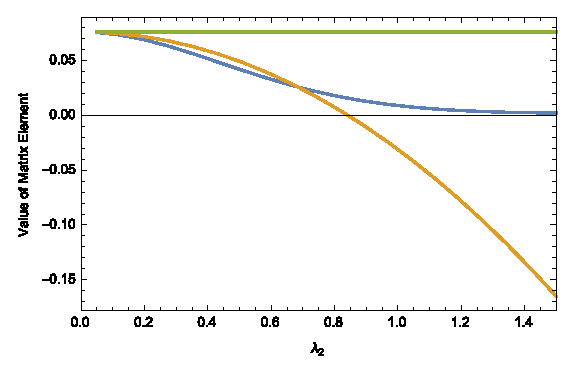
\includegraphics[width=0.6\textwidth]{LocalExpansion/Figures/ToyPotential000000} 
\caption{Matrix elements of $\braket{n'=0,\: l'=0,\: m_l'=0 | V | n=0,\: l=0,\: m_l=0}$ for $b=\lambda_1=1$ as a function of $\lambda_2$. The blue line shows the exact numerically evaluated matrix elements, while the orange line shows the second order Taylor approximation.
\label{fig:gaussToy1}}
\end{figure}

Matrix elements of the potential \eqref{eq:gaussToy} compare qualitatively as expected. First, we see that the exact values and the Taylor approximation converge for $\lambda_2\rightarrow 0$ in Figure \ref{fig:gaussToy1} but that the error increases as the range parameter $\lambda_2$ becomes non-perturbatively large. Figure \ref{fig:gaussToy2} demonstrates that the convergence is essentially independent of $\lambda_1$. Higher angular momenta are more difficult to integrate numerically, 

One interesting observation in the second order approximation is that the second derivative in $\lambda_2$ of the matrix elements is strictly negative for all of the channels tested, although this is not true for the exact results. Does the addition of fourth order terms (the third order terms are zero) introduce contributions which change this situation?

\begin{figure}[htb]
\centering 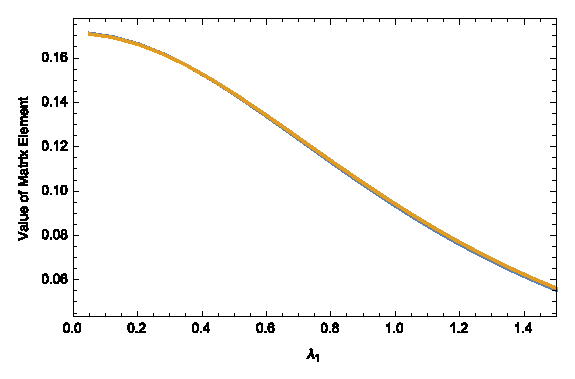
\includegraphics[width=0.6\textwidth]{LocalExpansion/Figures/ToyPotential000000l1} 
\caption{Matrix elements of $\braket{n'=0,\: l'=0,\: m_l'=0 | V | n=0,\: l=0,\: m_l=0}$ for $b=1$, $\lambda_2=0.05$ as a function of $\lambda_1$. The blue line shows the exact numerically evaluated matrix elements, while the orange line shows the second order Taylor approximation.
\label{fig:gaussToy2}}
\end{figure}



\end{section}
%%%%%%%%%%%%%%%%%%%%%%%%%%%%%%%%%%%%%%%%%%%%%%%%
\begin{section}{Comparison of nonlocal and local approximations to the in-medium effective term $V_D$ }

\end{section}
